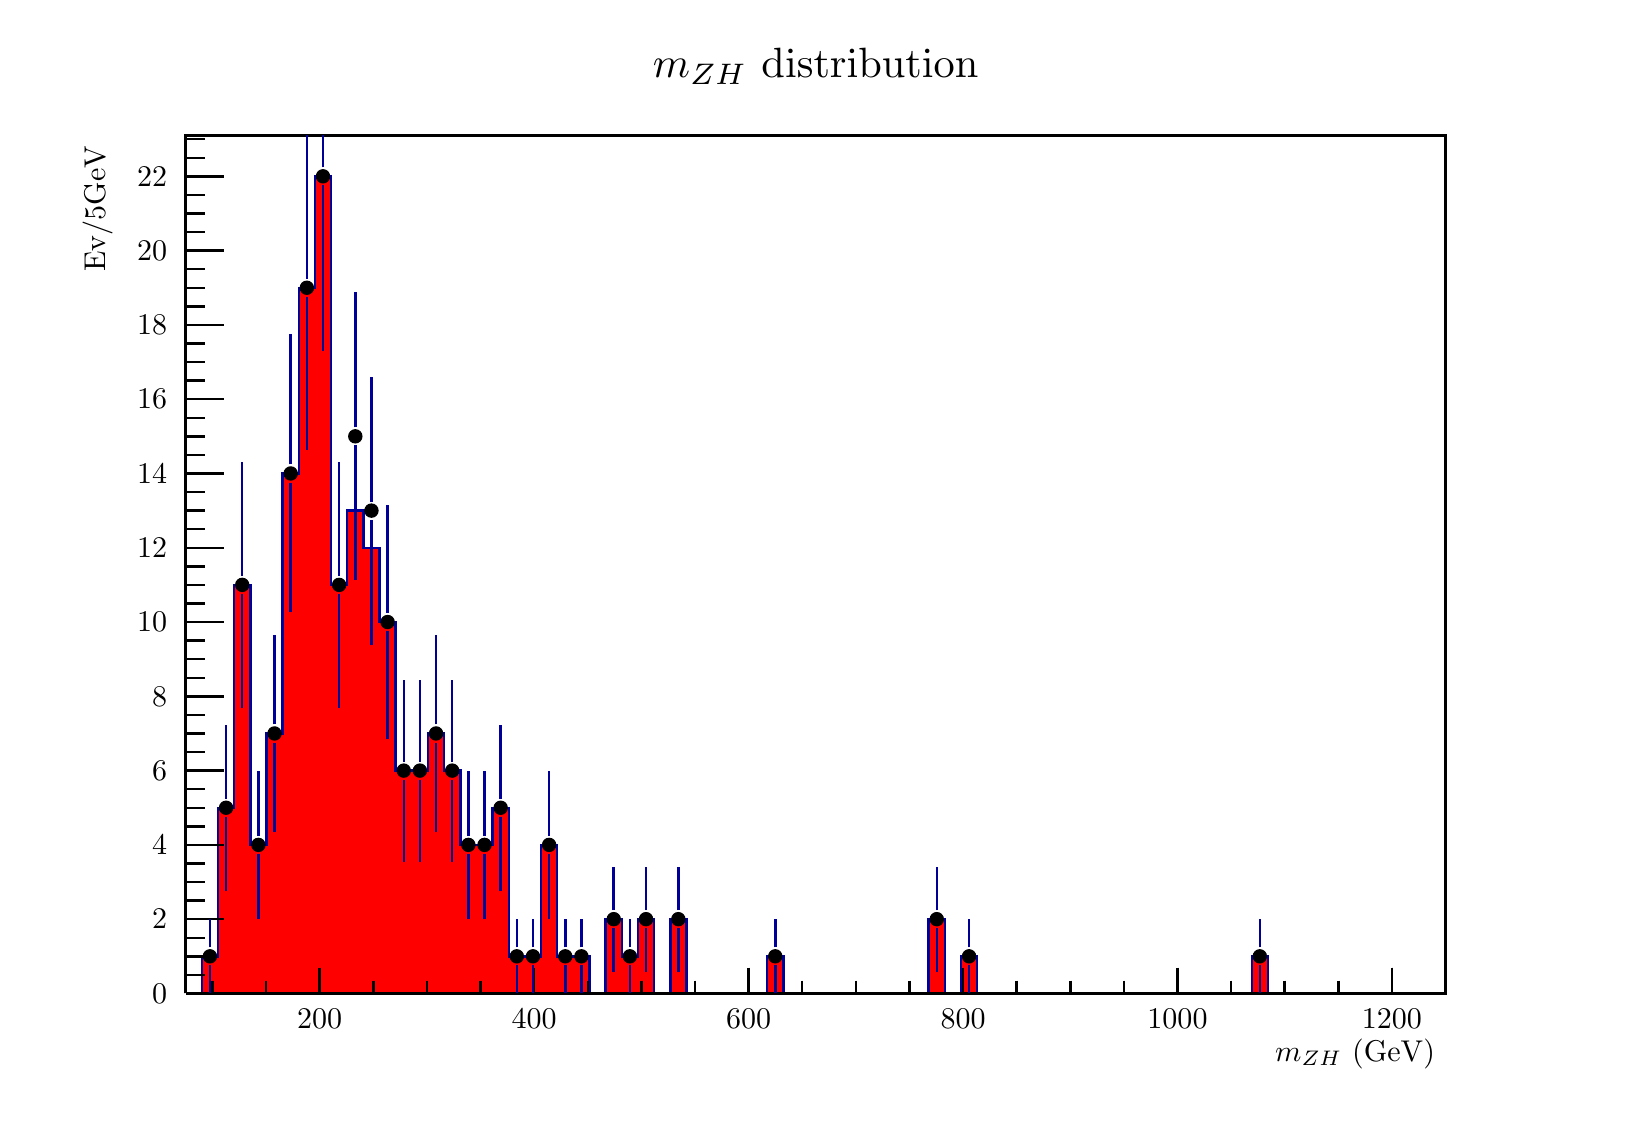
\begin{tikzpicture}
\pgfdeclareplotmark{cross} {
\pgfpathmoveto{\pgfpoint{-0.3\pgfplotmarksize}{\pgfplotmarksize}}
\pgfpathlineto{\pgfpoint{+0.3\pgfplotmarksize}{\pgfplotmarksize}}
\pgfpathlineto{\pgfpoint{+0.3\pgfplotmarksize}{0.3\pgfplotmarksize}}
\pgfpathlineto{\pgfpoint{+1\pgfplotmarksize}{0.3\pgfplotmarksize}}
\pgfpathlineto{\pgfpoint{+1\pgfplotmarksize}{-0.3\pgfplotmarksize}}
\pgfpathlineto{\pgfpoint{+0.3\pgfplotmarksize}{-0.3\pgfplotmarksize}}
\pgfpathlineto{\pgfpoint{+0.3\pgfplotmarksize}{-1.\pgfplotmarksize}}
\pgfpathlineto{\pgfpoint{-0.3\pgfplotmarksize}{-1.\pgfplotmarksize}}
\pgfpathlineto{\pgfpoint{-0.3\pgfplotmarksize}{-0.3\pgfplotmarksize}}
\pgfpathlineto{\pgfpoint{-1.\pgfplotmarksize}{-0.3\pgfplotmarksize}}
\pgfpathlineto{\pgfpoint{-1.\pgfplotmarksize}{0.3\pgfplotmarksize}}
\pgfpathlineto{\pgfpoint{-0.3\pgfplotmarksize}{0.3\pgfplotmarksize}}
\pgfpathclose
\pgfusepathqstroke
}
\pgfdeclareplotmark{cross*} {
\pgfpathmoveto{\pgfpoint{-0.3\pgfplotmarksize}{\pgfplotmarksize}}
\pgfpathlineto{\pgfpoint{+0.3\pgfplotmarksize}{\pgfplotmarksize}}
\pgfpathlineto{\pgfpoint{+0.3\pgfplotmarksize}{0.3\pgfplotmarksize}}
\pgfpathlineto{\pgfpoint{+1\pgfplotmarksize}{0.3\pgfplotmarksize}}
\pgfpathlineto{\pgfpoint{+1\pgfplotmarksize}{-0.3\pgfplotmarksize}}
\pgfpathlineto{\pgfpoint{+0.3\pgfplotmarksize}{-0.3\pgfplotmarksize}}
\pgfpathlineto{\pgfpoint{+0.3\pgfplotmarksize}{-1.\pgfplotmarksize}}
\pgfpathlineto{\pgfpoint{-0.3\pgfplotmarksize}{-1.\pgfplotmarksize}}
\pgfpathlineto{\pgfpoint{-0.3\pgfplotmarksize}{-0.3\pgfplotmarksize}}
\pgfpathlineto{\pgfpoint{-1.\pgfplotmarksize}{-0.3\pgfplotmarksize}}
\pgfpathlineto{\pgfpoint{-1.\pgfplotmarksize}{0.3\pgfplotmarksize}}
\pgfpathlineto{\pgfpoint{-0.3\pgfplotmarksize}{0.3\pgfplotmarksize}}
\pgfpathclose
\pgfusepathqfillstroke
}
\pgfdeclareplotmark{newstar} {
\pgfpathmoveto{\pgfqpoint{0pt}{\pgfplotmarksize}}
\pgfpathlineto{\pgfqpointpolar{44}{0.5\pgfplotmarksize}}
\pgfpathlineto{\pgfqpointpolar{18}{\pgfplotmarksize}}
\pgfpathlineto{\pgfqpointpolar{-20}{0.5\pgfplotmarksize}}
\pgfpathlineto{\pgfqpointpolar{-54}{\pgfplotmarksize}}
\pgfpathlineto{\pgfqpointpolar{-90}{0.5\pgfplotmarksize}}
\pgfpathlineto{\pgfqpointpolar{234}{\pgfplotmarksize}}
\pgfpathlineto{\pgfqpointpolar{198}{0.5\pgfplotmarksize}}
\pgfpathlineto{\pgfqpointpolar{162}{\pgfplotmarksize}}
\pgfpathlineto{\pgfqpointpolar{134}{0.5\pgfplotmarksize}}
\pgfpathclose
\pgfusepathqstroke
}
\pgfdeclareplotmark{newstar*} {
\pgfpathmoveto{\pgfqpoint{0pt}{\pgfplotmarksize}}
\pgfpathlineto{\pgfqpointpolar{44}{0.5\pgfplotmarksize}}
\pgfpathlineto{\pgfqpointpolar{18}{\pgfplotmarksize}}
\pgfpathlineto{\pgfqpointpolar{-20}{0.5\pgfplotmarksize}}
\pgfpathlineto{\pgfqpointpolar{-54}{\pgfplotmarksize}}
\pgfpathlineto{\pgfqpointpolar{-90}{0.5\pgfplotmarksize}}
\pgfpathlineto{\pgfqpointpolar{234}{\pgfplotmarksize}}
\pgfpathlineto{\pgfqpointpolar{198}{0.5\pgfplotmarksize}}
\pgfpathlineto{\pgfqpointpolar{162}{\pgfplotmarksize}}
\pgfpathlineto{\pgfqpointpolar{134}{0.5\pgfplotmarksize}}
\pgfpathclose
\pgfusepathqfillstroke
}
\definecolor{c}{rgb}{1,1,1};
\draw [color=c, fill=c] (0,0) rectangle (20,13.6207);
\draw [color=c, fill=c] (2,1.36207) rectangle (18,12.2586);
\definecolor{c}{rgb}{0,0,0};
\draw [c,line width=0.9] (2,1.36207) -- (2,12.2586) -- (18,12.2586) -- (18,1.36207) -- (2,1.36207);
\definecolor{c}{rgb}{1,1,1};
\draw [color=c, fill=c] (2,1.36207) rectangle (18,12.2586);
\definecolor{c}{rgb}{0,0,0};
\draw [c,line width=0.9] (2,1.36207) -- (2,12.2586) -- (18,12.2586) -- (18,1.36207) -- (2,1.36207);
\definecolor{c}{rgb}{1,0,0};
\draw [c, fill=c] (2,1.36207) -- (2,1.36207) -- (2.20513,1.36207) -- (2.20513,1.83378) -- (2.41026,1.83378) -- (2.41026,3.72063) -- (2.61538,3.72063) -- (2.61538,6.5509) -- (2.82051,6.5509) -- (2.82051,3.24892) -- (3.02564,3.24892) --
 (3.02564,4.66405) -- (3.23077,4.66405) -- (3.23077,7.96604) -- (3.4359,7.96604) -- (3.4359,10.3246) -- (3.64103,10.3246) -- (3.64103,11.7397) -- (3.84615,11.7397) -- (3.84615,6.5509) -- (4.05128,6.5509) -- (4.05128,7.49433) -- (4.25641,7.49433) --
 (4.25641,7.02261) -- (4.46154,7.02261) -- (4.46154,6.07919) -- (4.66667,6.07919) -- (4.66667,4.19234) -- (4.8718,4.19234) -- (4.8718,4.19234) -- (5.07692,4.19234) -- (5.07692,4.66405) -- (5.28205,4.66405) -- (5.28205,4.19234) -- (5.48718,4.19234) --
 (5.48718,3.24892) -- (5.69231,3.24892) -- (5.69231,3.24892) -- (5.89744,3.24892) -- (5.89744,3.72063) -- (6.10256,3.72063) -- (6.10256,1.83378) -- (6.30769,1.83378) -- (6.30769,1.83378) -- (6.51282,1.83378) -- (6.51282,3.24892) -- (6.71795,3.24892)
 -- (6.71795,1.83378) -- (6.92308,1.83378) -- (6.92308,1.83378) -- (7.12821,1.83378) -- (7.12821,1.36207) -- (7.33333,1.36207) -- (7.33333,2.30549) -- (7.53846,2.30549) -- (7.53846,1.83378) -- (7.74359,1.83378) -- (7.74359,2.30549) --
 (7.94872,2.30549) -- (7.94872,1.36207) -- (8.15385,1.36207) -- (8.15385,2.30549) -- (8.35897,2.30549) -- (8.35897,1.36207) -- (8.5641,1.36207) -- (8.5641,1.36207) -- (8.76923,1.36207) -- (8.76923,1.36207) -- (8.97436,1.36207) -- (8.97436,1.36207) --
 (9.17949,1.36207) -- (9.17949,1.36207) -- (9.38461,1.36207) -- (9.38461,1.83378) -- (9.58974,1.83378) -- (9.58974,1.36207) -- (9.79487,1.36207) -- (9.79487,1.36207) -- (10,1.36207) -- (10,1.36207) -- (10.2051,1.36207) -- (10.2051,1.36207) --
 (10.4103,1.36207) -- (10.4103,1.36207) -- (10.6154,1.36207) -- (10.6154,1.36207) -- (10.8205,1.36207) -- (10.8205,1.36207) -- (11.0256,1.36207) -- (11.0256,1.36207) -- (11.2308,1.36207) -- (11.2308,1.36207) -- (11.4359,1.36207) -- (11.4359,2.30549)
 -- (11.641,2.30549) -- (11.641,1.36207) -- (11.8462,1.36207) -- (11.8462,1.83378) -- (12.0513,1.83378) -- (12.0513,1.36207) -- (12.2564,1.36207) -- (12.2564,1.36207) -- (12.4615,1.36207) -- (12.4615,1.36207) -- (12.6667,1.36207) -- (12.6667,1.36207)
 -- (12.8718,1.36207) -- (12.8718,1.36207) -- (13.0769,1.36207) -- (13.0769,1.36207) -- (13.2821,1.36207) -- (13.2821,1.36207) -- (13.4872,1.36207) -- (13.4872,1.36207) -- (13.6923,1.36207) -- (13.6923,1.36207) -- (13.8974,1.36207) --
 (13.8974,1.36207) -- (14.1026,1.36207) -- (14.1026,1.36207) -- (14.3077,1.36207) -- (14.3077,1.36207) -- (14.5128,1.36207) -- (14.5128,1.36207) -- (14.7179,1.36207) -- (14.7179,1.36207) -- (14.9231,1.36207) -- (14.9231,1.36207) -- (15.1282,1.36207)
 -- (15.1282,1.36207) -- (15.3333,1.36207) -- (15.3333,1.36207) -- (15.5385,1.36207) -- (15.5385,1.83378) -- (15.7436,1.83378) -- (15.7436,1.36207) -- (15.9487,1.36207) -- (15.9487,1.36207) -- (16.1538,1.36207) -- (16.1538,1.36207) --
 (16.359,1.36207) -- (16.359,1.36207) -- (16.5641,1.36207) -- (16.5641,1.36207) -- (16.7692,1.36207) -- (16.7692,1.36207) -- (16.9744,1.36207) -- (16.9744,1.36207) -- (17.1795,1.36207) -- (17.1795,1.36207) -- (17.3846,1.36207) -- (17.3846,1.36207) --
 (17.5897,1.36207) -- (17.5897,1.36207) -- (17.7949,1.36207) -- (17.7949,1.36207) -- (18,1.36207) -- (18,1.36207);
\definecolor{c}{rgb}{0,0,0.6};
\draw [c,line width=0.9] (2,1.36207) -- (2.20513,1.36207) -- (2.20513,1.83378) -- (2.41026,1.83378) -- (2.41026,3.72063) -- (2.61538,3.72063) -- (2.61538,6.5509) -- (2.82051,6.5509) -- (2.82051,3.24892) -- (3.02564,3.24892) -- (3.02564,4.66405) --
 (3.23077,4.66405) -- (3.23077,7.96604) -- (3.4359,7.96604) -- (3.4359,10.3246) -- (3.64103,10.3246) -- (3.64103,11.7397) -- (3.84615,11.7397) -- (3.84615,6.5509) -- (4.05128,6.5509) -- (4.05128,7.49433) -- (4.25641,7.49433) -- (4.25641,7.02261) --
 (4.46154,7.02261) -- (4.46154,6.07919) -- (4.66667,6.07919) -- (4.66667,4.19234) -- (4.8718,4.19234) -- (4.8718,4.19234) -- (5.07692,4.19234) -- (5.07692,4.66405) -- (5.28205,4.66405) -- (5.28205,4.19234) -- (5.48718,4.19234) -- (5.48718,3.24892) --
 (5.69231,3.24892) -- (5.69231,3.24892) -- (5.89744,3.24892) -- (5.89744,3.72063) -- (6.10256,3.72063) -- (6.10256,1.83378) -- (6.30769,1.83378) -- (6.30769,1.83378) -- (6.51282,1.83378) -- (6.51282,3.24892) -- (6.71795,3.24892) -- (6.71795,1.83378)
 -- (6.92308,1.83378) -- (6.92308,1.83378) -- (7.12821,1.83378) -- (7.12821,1.36207) -- (7.33333,1.36207) -- (7.33333,2.30549) -- (7.53846,2.30549) -- (7.53846,1.83378) -- (7.74359,1.83378) -- (7.74359,2.30549) -- (7.94872,2.30549) --
 (7.94872,1.36207) -- (8.15385,1.36207) -- (8.15385,2.30549) -- (8.35897,2.30549) -- (8.35897,1.36207) -- (8.5641,1.36207) -- (8.5641,1.36207) -- (8.76923,1.36207) -- (8.76923,1.36207) -- (8.97436,1.36207) -- (8.97436,1.36207) -- (9.17949,1.36207) --
 (9.17949,1.36207) -- (9.38461,1.36207) -- (9.38461,1.83378) -- (9.58974,1.83378) -- (9.58974,1.36207) -- (9.79487,1.36207) -- (9.79487,1.36207) -- (10,1.36207) -- (10,1.36207) -- (10.2051,1.36207) -- (10.2051,1.36207) -- (10.4103,1.36207) --
 (10.4103,1.36207) -- (10.6154,1.36207) -- (10.6154,1.36207) -- (10.8205,1.36207) -- (10.8205,1.36207) -- (11.0256,1.36207) -- (11.0256,1.36207) -- (11.2308,1.36207) -- (11.2308,1.36207) -- (11.4359,1.36207) -- (11.4359,2.30549) -- (11.641,2.30549)
 -- (11.641,1.36207) -- (11.8462,1.36207) -- (11.8462,1.83378) -- (12.0513,1.83378) -- (12.0513,1.36207) -- (12.2564,1.36207) -- (12.2564,1.36207) -- (12.4615,1.36207) -- (12.4615,1.36207) -- (12.6667,1.36207) -- (12.6667,1.36207) --
 (12.8718,1.36207) -- (12.8718,1.36207) -- (13.0769,1.36207) -- (13.0769,1.36207) -- (13.2821,1.36207) -- (13.2821,1.36207) -- (13.4872,1.36207) -- (13.4872,1.36207) -- (13.6923,1.36207) -- (13.6923,1.36207) -- (13.8974,1.36207) -- (13.8974,1.36207)
 -- (14.1026,1.36207) -- (14.1026,1.36207) -- (14.3077,1.36207) -- (14.3077,1.36207) -- (14.5128,1.36207) -- (14.5128,1.36207) -- (14.7179,1.36207) -- (14.7179,1.36207) -- (14.9231,1.36207) -- (14.9231,1.36207) -- (15.1282,1.36207) --
 (15.1282,1.36207) -- (15.3333,1.36207) -- (15.3333,1.36207) -- (15.5385,1.36207) -- (15.5385,1.83378) -- (15.7436,1.83378) -- (15.7436,1.36207) -- (15.9487,1.36207) -- (15.9487,1.36207) -- (16.1538,1.36207) -- (16.1538,1.36207) -- (16.359,1.36207)
 -- (16.359,1.36207) -- (16.5641,1.36207) -- (16.5641,1.36207) -- (16.7692,1.36207) -- (16.7692,1.36207) -- (16.9744,1.36207) -- (16.9744,1.36207) -- (17.1795,1.36207) -- (17.1795,1.36207) -- (17.3846,1.36207) -- (17.3846,1.36207) --
 (17.5897,1.36207) -- (17.5897,1.36207) -- (17.7949,1.36207) -- (17.7949,1.36207) -- (18,1.36207);
\definecolor{c}{rgb}{0,0,0};
\draw [c,line width=0.9] (2,1.36207) -- (18,1.36207);
\draw [anchor= east] (18,0.599311) node[scale=1.08496, color=c, rotate=0]{$m_{ZH} \mbox{ (GeV)}$};
\draw [c,line width=0.9] (3.70213,1.68897) -- (3.70213,1.36207);
\draw [c,line width=0.9] (4.38298,1.52552) -- (4.38298,1.36207);
\draw [c,line width=0.9] (5.06383,1.52552) -- (5.06383,1.36207);
\draw [c,line width=0.9] (5.74468,1.52552) -- (5.74468,1.36207);
\draw [c,line width=0.9] (6.42553,1.68897) -- (6.42553,1.36207);
\draw [c,line width=0.9] (7.10638,1.52552) -- (7.10638,1.36207);
\draw [c,line width=0.9] (7.78723,1.52552) -- (7.78723,1.36207);
\draw [c,line width=0.9] (8.46809,1.52552) -- (8.46809,1.36207);
\draw [c,line width=0.9] (9.14894,1.68897) -- (9.14894,1.36207);
\draw [c,line width=0.9] (9.82979,1.52552) -- (9.82979,1.36207);
\draw [c,line width=0.9] (10.5106,1.52552) -- (10.5106,1.36207);
\draw [c,line width=0.9] (11.1915,1.52552) -- (11.1915,1.36207);
\draw [c,line width=0.9] (11.8723,1.68897) -- (11.8723,1.36207);
\draw [c,line width=0.9] (12.5532,1.52552) -- (12.5532,1.36207);
\draw [c,line width=0.9] (13.234,1.52552) -- (13.234,1.36207);
\draw [c,line width=0.9] (13.9149,1.52552) -- (13.9149,1.36207);
\draw [c,line width=0.9] (14.5957,1.68897) -- (14.5957,1.36207);
\draw [c,line width=0.9] (15.2766,1.52552) -- (15.2766,1.36207);
\draw [c,line width=0.9] (15.9574,1.52552) -- (15.9574,1.36207);
\draw [c,line width=0.9] (16.6383,1.52552) -- (16.6383,1.36207);
\draw [c,line width=0.9] (17.3191,1.68897) -- (17.3191,1.36207);
\draw [c,line width=0.9] (3.70213,1.68897) -- (3.70213,1.36207);
\draw [c,line width=0.9] (3.02128,1.52552) -- (3.02128,1.36207);
\draw [c,line width=0.9] (2.34043,1.52552) -- (2.34043,1.36207);
\draw [c,line width=0.9] (17.3191,1.68897) -- (17.3191,1.36207);
\draw [c,line width=0.9] (18,1.52552) -- (18,1.36207);
\draw [anchor=base] (3.70213,0.912586) node[scale=1.08496, color=c, rotate=0]{200};
\draw [anchor=base] (6.42553,0.912586) node[scale=1.08496, color=c, rotate=0]{400};
\draw [anchor=base] (9.14894,0.912586) node[scale=1.08496, color=c, rotate=0]{600};
\draw [anchor=base] (11.8723,0.912586) node[scale=1.08496, color=c, rotate=0]{800};
\draw [anchor=base] (14.5957,0.912586) node[scale=1.08496, color=c, rotate=0]{1000};
\draw [anchor=base] (17.3191,0.912586) node[scale=1.08496, color=c, rotate=0]{1200};
\draw [c,line width=0.9] (2,1.36207) -- (2,12.2586);
\draw [anchor= east] (0.88,12.2586) node[scale=1.08496, color=c, rotate=90]{$\mbox{Ev/5GeV}$};
\draw [c,line width=0.9] (2.48,1.36207) -- (2,1.36207);
\draw [c,line width=0.9] (2.24,1.59793) -- (2,1.59793);
\draw [c,line width=0.9] (2.24,1.83378) -- (2,1.83378);
\draw [c,line width=0.9] (2.24,2.06964) -- (2,2.06964);
\draw [c,line width=0.9] (2.48,2.30549) -- (2,2.30549);
\draw [c,line width=0.9] (2.24,2.54135) -- (2,2.54135);
\draw [c,line width=0.9] (2.24,2.77721) -- (2,2.77721);
\draw [c,line width=0.9] (2.24,3.01306) -- (2,3.01306);
\draw [c,line width=0.9] (2.48,3.24892) -- (2,3.24892);
\draw [c,line width=0.9] (2.24,3.48477) -- (2,3.48477);
\draw [c,line width=0.9] (2.24,3.72063) -- (2,3.72063);
\draw [c,line width=0.9] (2.24,3.95649) -- (2,3.95649);
\draw [c,line width=0.9] (2.48,4.19234) -- (2,4.19234);
\draw [c,line width=0.9] (2.24,4.4282) -- (2,4.4282);
\draw [c,line width=0.9] (2.24,4.66405) -- (2,4.66405);
\draw [c,line width=0.9] (2.24,4.89991) -- (2,4.89991);
\draw [c,line width=0.9] (2.48,5.13577) -- (2,5.13577);
\draw [c,line width=0.9] (2.24,5.37162) -- (2,5.37162);
\draw [c,line width=0.9] (2.24,5.60748) -- (2,5.60748);
\draw [c,line width=0.9] (2.24,5.84333) -- (2,5.84333);
\draw [c,line width=0.9] (2.48,6.07919) -- (2,6.07919);
\draw [c,line width=0.9] (2.24,6.31505) -- (2,6.31505);
\draw [c,line width=0.9] (2.24,6.5509) -- (2,6.5509);
\draw [c,line width=0.9] (2.24,6.78676) -- (2,6.78676);
\draw [c,line width=0.9] (2.48,7.02261) -- (2,7.02261);
\draw [c,line width=0.9] (2.24,7.25847) -- (2,7.25847);
\draw [c,line width=0.9] (2.24,7.49433) -- (2,7.49433);
\draw [c,line width=0.9] (2.24,7.73018) -- (2,7.73018);
\draw [c,line width=0.9] (2.48,7.96604) -- (2,7.96604);
\draw [c,line width=0.9] (2.24,8.2019) -- (2,8.2019);
\draw [c,line width=0.9] (2.24,8.43775) -- (2,8.43775);
\draw [c,line width=0.9] (2.24,8.67361) -- (2,8.67361);
\draw [c,line width=0.9] (2.48,8.90946) -- (2,8.90946);
\draw [c,line width=0.9] (2.24,9.14532) -- (2,9.14532);
\draw [c,line width=0.9] (2.24,9.38118) -- (2,9.38118);
\draw [c,line width=0.9] (2.24,9.61703) -- (2,9.61703);
\draw [c,line width=0.9] (2.48,9.85289) -- (2,9.85289);
\draw [c,line width=0.9] (2.24,10.0887) -- (2,10.0887);
\draw [c,line width=0.9] (2.24,10.3246) -- (2,10.3246);
\draw [c,line width=0.9] (2.24,10.5605) -- (2,10.5605);
\draw [c,line width=0.9] (2.48,10.7963) -- (2,10.7963);
\draw [c,line width=0.9] (2.24,11.0322) -- (2,11.0322);
\draw [c,line width=0.9] (2.24,11.268) -- (2,11.268);
\draw [c,line width=0.9] (2.24,11.5039) -- (2,11.5039);
\draw [c,line width=0.9] (2.48,11.7397) -- (2,11.7397);
\draw [c,line width=0.9] (2.48,11.7397) -- (2,11.7397);
\draw [c,line width=0.9] (2.24,11.9756) -- (2,11.9756);
\draw [c,line width=0.9] (2.24,12.2114) -- (2,12.2114);
\draw [anchor= east] (1.9,1.36207) node[scale=1.08496, color=c, rotate=0]{0};
\draw [anchor= east] (1.9,2.30549) node[scale=1.08496, color=c, rotate=0]{2};
\draw [anchor= east] (1.9,3.24892) node[scale=1.08496, color=c, rotate=0]{4};
\draw [anchor= east] (1.9,4.19234) node[scale=1.08496, color=c, rotate=0]{6};
\draw [anchor= east] (1.9,5.13577) node[scale=1.08496, color=c, rotate=0]{8};
\draw [anchor= east] (1.9,6.07919) node[scale=1.08496, color=c, rotate=0]{10};
\draw [anchor= east] (1.9,7.02261) node[scale=1.08496, color=c, rotate=0]{12};
\draw [anchor= east] (1.9,7.96604) node[scale=1.08496, color=c, rotate=0]{14};
\draw [anchor= east] (1.9,8.90946) node[scale=1.08496, color=c, rotate=0]{16};
\draw [anchor= east] (1.9,9.85289) node[scale=1.08496, color=c, rotate=0]{18};
\draw [anchor= east] (1.9,10.7963) node[scale=1.08496, color=c, rotate=0]{20};
\draw [anchor= east] (1.9,11.7397) node[scale=1.08496, color=c, rotate=0]{22};
\definecolor{c}{rgb}{0,0,0.6};
\draw [c,line width=0.9] (2.30769,1.36207) -- (2.30769,1.71884);
\draw [c,line width=0.9] (2.30769,1.94872) -- (2.30769,2.30549);
\definecolor{c}{rgb}{0,0,0};
\foreach \P in {(2.30769,1.83378)}{\draw[mark options={color=c,fill=c},mark size=2.402402pt,mark=*] plot coordinates {\P};}
\definecolor{c}{rgb}{0,0,0.6};
\draw [c,line width=0.9] (2.51282,2.66585) -- (2.51282,3.60569);
\draw [c,line width=0.9] (2.51282,3.83557) -- (2.51282,4.77541);
\definecolor{c}{rgb}{0,0,0};
\foreach \P in {(2.51282,3.72063)}{\draw[mark options={color=c,fill=c},mark size=2.402402pt,mark=*] plot coordinates {\P};}
\definecolor{c}{rgb}{0,0,0.6};
\draw [c,line width=0.9] (2.71795,4.98641) -- (2.71795,6.43596);
\draw [c,line width=0.9] (2.71795,6.66585) -- (2.71795,8.1154);
\definecolor{c}{rgb}{0,0,0};
\foreach \P in {(2.71795,6.5509)}{\draw[mark options={color=c,fill=c},mark size=2.402402pt,mark=*] plot coordinates {\P};}
\definecolor{c}{rgb}{0,0,0.6};
\draw [c,line width=0.9] (2.92308,2.30549) -- (2.92308,3.13398);
\draw [c,line width=0.9] (2.92308,3.36386) -- (2.92308,4.19234);
\definecolor{c}{rgb}{0,0,0};
\foreach \P in {(2.92308,3.24892)}{\draw[mark options={color=c,fill=c},mark size=2.402402pt,mark=*] plot coordinates {\P};}
\definecolor{c}{rgb}{0,0,0.6};
\draw [c,line width=0.9] (3.12821,3.41602) -- (3.12821,4.54911);
\draw [c,line width=0.9] (3.12821,4.779) -- (3.12821,5.91209);
\definecolor{c}{rgb}{0,0,0};
\foreach \P in {(3.12821,4.66405)}{\draw[mark options={color=c,fill=c},mark size=2.402402pt,mark=*] plot coordinates {\P};}
\definecolor{c}{rgb}{0,0,0.6};
\draw [c,line width=0.9] (3.33333,6.20105) -- (3.33333,7.8511);
\draw [c,line width=0.9] (3.33333,8.08098) -- (3.33333,9.73102);
\definecolor{c}{rgb}{0,0,0};
\foreach \P in {(3.33333,7.96604)}{\draw[mark options={color=c,fill=c},mark size=2.402402pt,mark=*] plot coordinates {\P};}
\definecolor{c}{rgb}{0,0,0.6};
\draw [c,line width=0.9] (3.53846,8.26845) -- (3.53846,10.2097);
\draw [c,line width=0.9] (3.53846,10.4395) -- (3.53846,12.2586);
\definecolor{c}{rgb}{0,0,0};
\foreach \P in {(3.53846,10.3246)}{\draw[mark options={color=c,fill=c},mark size=2.402402pt,mark=*] plot coordinates {\P};}
\definecolor{c}{rgb}{0,0,0.6};
\draw [c,line width=0.9] (3.74359,9.52721) -- (3.74359,11.6248);
\draw [c,line width=0.9] (3.74359,11.8547) -- (3.74359,12.2586);
\definecolor{c}{rgb}{0,0,0};
\foreach \P in {(3.74359,11.7397)}{\draw[mark options={color=c,fill=c},mark size=2.402402pt,mark=*] plot coordinates {\P};}
\definecolor{c}{rgb}{0,0,0.6};
\draw [c,line width=0.9] (3.94872,4.98641) -- (3.94872,6.43596);
\draw [c,line width=0.9] (3.94872,6.66585) -- (3.94872,8.1154);
\definecolor{c}{rgb}{0,0,0};
\foreach \P in {(3.94872,6.5509)}{\draw[mark options={color=c,fill=c},mark size=2.402402pt,mark=*] plot coordinates {\P};}
\definecolor{c}{rgb}{0,0,0.6};
\draw [c,line width=0.9] (4.15385,6.61082) -- (4.15385,8.32281);
\draw [c,line width=0.9] (4.15385,8.55269) -- (4.15385,10.2647);
\definecolor{c}{rgb}{0,0,0};
\foreach \P in {(4.15385,8.43775)}{\draw[mark options={color=c,fill=c},mark size=2.402402pt,mark=*] plot coordinates {\P};}
\definecolor{c}{rgb}{0,0,0.6};
\draw [c,line width=0.9] (4.35897,5.79354) -- (4.35897,7.37938);
\draw [c,line width=0.9] (4.35897,7.60927) -- (4.35897,9.19511);
\definecolor{c}{rgb}{0,0,0};
\foreach \P in {(4.35897,7.49433)}{\draw[mark options={color=c,fill=c},mark size=2.402402pt,mark=*] plot coordinates {\P};}
\definecolor{c}{rgb}{0,0,0.6};
\draw [c,line width=0.9] (4.5641,4.58751) -- (4.5641,5.96425);
\draw [c,line width=0.9] (4.5641,6.19413) -- (4.5641,7.57088);
\definecolor{c}{rgb}{0,0,0};
\foreach \P in {(4.5641,6.07919)}{\draw[mark options={color=c,fill=c},mark size=2.402402pt,mark=*] plot coordinates {\P};}
\definecolor{c}{rgb}{0,0,0.6};
\draw [c,line width=0.9] (4.76923,3.03689) -- (4.76923,4.0774);
\draw [c,line width=0.9] (4.76923,4.30728) -- (4.76923,5.3478);
\definecolor{c}{rgb}{0,0,0};
\foreach \P in {(4.76923,4.19234)}{\draw[mark options={color=c,fill=c},mark size=2.402402pt,mark=*] plot coordinates {\P};}
\definecolor{c}{rgb}{0,0,0.6};
\draw [c,line width=0.9] (4.97436,3.03689) -- (4.97436,4.0774);
\draw [c,line width=0.9] (4.97436,4.30728) -- (4.97436,5.3478);
\definecolor{c}{rgb}{0,0,0};
\foreach \P in {(4.97436,4.19234)}{\draw[mark options={color=c,fill=c},mark size=2.402402pt,mark=*] plot coordinates {\P};}
\definecolor{c}{rgb}{0,0,0.6};
\draw [c,line width=0.9] (5.17949,3.41602) -- (5.17949,4.54911);
\draw [c,line width=0.9] (5.17949,4.779) -- (5.17949,5.91209);
\definecolor{c}{rgb}{0,0,0};
\foreach \P in {(5.17949,4.66405)}{\draw[mark options={color=c,fill=c},mark size=2.402402pt,mark=*] plot coordinates {\P};}
\definecolor{c}{rgb}{0,0,0.6};
\draw [c,line width=0.9] (5.38462,3.03689) -- (5.38462,4.0774);
\draw [c,line width=0.9] (5.38462,4.30728) -- (5.38462,5.3478);
\definecolor{c}{rgb}{0,0,0};
\foreach \P in {(5.38462,4.19234)}{\draw[mark options={color=c,fill=c},mark size=2.402402pt,mark=*] plot coordinates {\P};}
\definecolor{c}{rgb}{0,0,0.6};
\draw [c,line width=0.9] (5.58974,2.30549) -- (5.58974,3.13398);
\draw [c,line width=0.9] (5.58974,3.36386) -- (5.58974,4.19234);
\definecolor{c}{rgb}{0,0,0};
\foreach \P in {(5.58974,3.24892)}{\draw[mark options={color=c,fill=c},mark size=2.402402pt,mark=*] plot coordinates {\P};}
\definecolor{c}{rgb}{0,0,0.6};
\draw [c,line width=0.9] (5.79487,2.30549) -- (5.79487,3.13398);
\draw [c,line width=0.9] (5.79487,3.36386) -- (5.79487,4.19234);
\definecolor{c}{rgb}{0,0,0};
\foreach \P in {(5.79487,3.24892)}{\draw[mark options={color=c,fill=c},mark size=2.402402pt,mark=*] plot coordinates {\P};}
\definecolor{c}{rgb}{0,0,0.6};
\draw [c,line width=0.9] (6,2.66585) -- (6,3.60569);
\draw [c,line width=0.9] (6,3.83557) -- (6,4.77541);
\definecolor{c}{rgb}{0,0,0};
\foreach \P in {(6,3.72063)}{\draw[mark options={color=c,fill=c},mark size=2.402402pt,mark=*] plot coordinates {\P};}
\definecolor{c}{rgb}{0,0,0.6};
\draw [c,line width=0.9] (6.20513,1.36207) -- (6.20513,1.71884);
\draw [c,line width=0.9] (6.20513,1.94872) -- (6.20513,2.30549);
\definecolor{c}{rgb}{0,0,0};
\foreach \P in {(6.20513,1.83378)}{\draw[mark options={color=c,fill=c},mark size=2.402402pt,mark=*] plot coordinates {\P};}
\definecolor{c}{rgb}{0,0,0.6};
\draw [c,line width=0.9] (6.41026,1.36207) -- (6.41026,1.71884);
\draw [c,line width=0.9] (6.41026,1.94872) -- (6.41026,2.30549);
\definecolor{c}{rgb}{0,0,0};
\foreach \P in {(6.41026,1.83378)}{\draw[mark options={color=c,fill=c},mark size=2.402402pt,mark=*] plot coordinates {\P};}
\definecolor{c}{rgb}{0,0,0.6};
\draw [c,line width=0.9] (6.61538,2.30549) -- (6.61538,3.13398);
\draw [c,line width=0.9] (6.61538,3.36386) -- (6.61538,4.19234);
\definecolor{c}{rgb}{0,0,0};
\foreach \P in {(6.61538,3.24892)}{\draw[mark options={color=c,fill=c},mark size=2.402402pt,mark=*] plot coordinates {\P};}
\definecolor{c}{rgb}{0,0,0.6};
\draw [c,line width=0.9] (6.82051,1.36207) -- (6.82051,1.71884);
\draw [c,line width=0.9] (6.82051,1.94872) -- (6.82051,2.30549);
\definecolor{c}{rgb}{0,0,0};
\foreach \P in {(6.82051,1.83378)}{\draw[mark options={color=c,fill=c},mark size=2.402402pt,mark=*] plot coordinates {\P};}
\definecolor{c}{rgb}{0,0,0.6};
\draw [c,line width=0.9] (7.02564,1.36207) -- (7.02564,1.71884);
\draw [c,line width=0.9] (7.02564,1.94872) -- (7.02564,2.30549);
\definecolor{c}{rgb}{0,0,0};
\foreach \P in {(7.02564,1.83378)}{\draw[mark options={color=c,fill=c},mark size=2.402402pt,mark=*] plot coordinates {\P};}
\definecolor{c}{rgb}{0,0,0.6};
\draw [c,line width=0.9] (7.4359,1.63839) -- (7.4359,2.19055);
\draw [c,line width=0.9] (7.4359,2.42044) -- (7.4359,2.9726);
\definecolor{c}{rgb}{0,0,0};
\foreach \P in {(7.4359,2.30549)}{\draw[mark options={color=c,fill=c},mark size=2.402402pt,mark=*] plot coordinates {\P};}
\definecolor{c}{rgb}{0,0,0.6};
\draw [c,line width=0.9] (7.64103,1.36207) -- (7.64103,1.71884);
\draw [c,line width=0.9] (7.64103,1.94872) -- (7.64103,2.30549);
\definecolor{c}{rgb}{0,0,0};
\foreach \P in {(7.64103,1.83378)}{\draw[mark options={color=c,fill=c},mark size=2.402402pt,mark=*] plot coordinates {\P};}
\definecolor{c}{rgb}{0,0,0.6};
\draw [c,line width=0.9] (7.84615,1.63839) -- (7.84615,2.19055);
\draw [c,line width=0.9] (7.84615,2.42044) -- (7.84615,2.9726);
\definecolor{c}{rgb}{0,0,0};
\foreach \P in {(7.84615,2.30549)}{\draw[mark options={color=c,fill=c},mark size=2.402402pt,mark=*] plot coordinates {\P};}
\definecolor{c}{rgb}{0,0,0.6};
\draw [c,line width=0.9] (8.25641,1.63839) -- (8.25641,2.19055);
\draw [c,line width=0.9] (8.25641,2.42044) -- (8.25641,2.9726);
\definecolor{c}{rgb}{0,0,0};
\foreach \P in {(8.25641,2.30549)}{\draw[mark options={color=c,fill=c},mark size=2.402402pt,mark=*] plot coordinates {\P};}
\definecolor{c}{rgb}{0,0,0.6};
\draw [c,line width=0.9] (9.48718,1.36207) -- (9.48718,1.71884);
\draw [c,line width=0.9] (9.48718,1.94872) -- (9.48718,2.30549);
\definecolor{c}{rgb}{0,0,0};
\foreach \P in {(9.48718,1.83378)}{\draw[mark options={color=c,fill=c},mark size=2.402402pt,mark=*] plot coordinates {\P};}
\definecolor{c}{rgb}{0,0,0.6};
\draw [c,line width=0.9] (11.5385,1.63839) -- (11.5385,2.19055);
\draw [c,line width=0.9] (11.5385,2.42044) -- (11.5385,2.9726);
\definecolor{c}{rgb}{0,0,0};
\foreach \P in {(11.5385,2.30549)}{\draw[mark options={color=c,fill=c},mark size=2.402402pt,mark=*] plot coordinates {\P};}
\definecolor{c}{rgb}{0,0,0.6};
\draw [c,line width=0.9] (11.9487,1.36207) -- (11.9487,1.71884);
\draw [c,line width=0.9] (11.9487,1.94872) -- (11.9487,2.30549);
\definecolor{c}{rgb}{0,0,0};
\foreach \P in {(11.9487,1.83378)}{\draw[mark options={color=c,fill=c},mark size=2.402402pt,mark=*] plot coordinates {\P};}
\definecolor{c}{rgb}{0,0,0.6};
\draw [c,line width=0.9] (15.641,1.36207) -- (15.641,1.71884);
\draw [c,line width=0.9] (15.641,1.94872) -- (15.641,2.30549);
\definecolor{c}{rgb}{0,0,0};
\foreach \P in {(15.641,1.83378)}{\draw[mark options={color=c,fill=c},mark size=2.402402pt,mark=*] plot coordinates {\P};}
\draw (10,13.1388) node[scale=1.5317, color=c, rotate=0]{$m_{ZH} \mbox{ distribution}$};
\end{tikzpicture}
